\chapter{Обзор предметной области}
\label{chapter1}

\section{Подготовка и предобработка данных. Формальное
задание проблемы}
\label{problem}

Рассмотрим, вкратце, весь процесс построения карты глубины: от непосредственной фотосъемки до получения итогового результата.

Для простоты мы будем считать, что у нас есть две камеры ($C_1$~и~$C_2$), 
которые снимают одну и ту же сцену одновременно, но из различных точек 
обзора. Камеры делают два снимка, и мы получаем, соответственно, две 
фотографии одной и той же сцены.  Пример таких снимков можно увидеть на рис. \ref{pic:1}.

\begin{figure}[h!]
\center{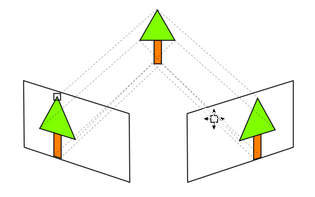
\includegraphics[scale=1.5]{1.png}}
\caption{Снимки "стрелки" с двух ракурсов}
\label{pic:1}
\end{figure}

Следующим шагом необходимо сопоставить каждую точку левого 
изображения соответствующей ей точку на правом изображении. Эта 
проблема получила название проблема соответствия. На рис. \ref{pic:1}
изображено пространство поиска подходящей точки – это все правое 
изображение, то есть мы вынуждены производить наш поиск в двух 
измерениях. Для упрощения задачи поиска соответствий производится ректификация: изображения корректируются так, что соответствующие точки находятся на одной строчке.  После ректификации наши изображения станут выглядеть так:

\begin{figure}[h!]
\center{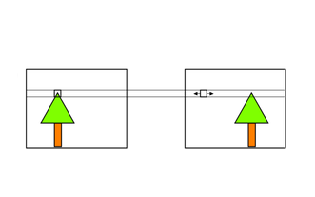
\includegraphics[scale=1.5]{2.png}}
\caption{Ректифицированные снимки "стрелки" с двух ракурсов. Пространство поиска сужено до 
одной строчки.}
\label{pic:2}
\end{figure}

Ректификация позволяет сузить пространство поиска решений для 
проблемы соответствия до одного измерения. Более конкретно, после 
проведения ректификации, все «подозрительные» пиксели, то есть все 
пиксели правого изображения, которые могут соответствовать данной точке 
левой картинки, будут находиться в одной строчке. Именно пара 
ректифицированных изображений является входными параметрами к задаче 
восстановления глубины. 

Следующим глобальным этапом является решение проблемы 
соответствия, а именно, построение карты диспаратности (disparity map) по 
двум ректифицированным изображениям. Для того чтобы понять что такое 
карта диспаратности рассмотрим следующий пример:

\begin{figure}[h!]
\center{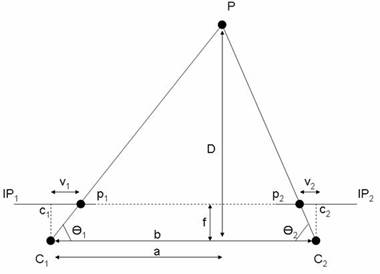
\includegraphics[scale=1.5]{3.jpg}}
\caption{Геометрическое представление наблюдаемой сцены.}
\label{pic:3}
\end{figure}

  Тогда $C_1$ и $C_2$ – это центры камер. $IP_1$ и $IP_2$ – это плоскости изображения, то 
есть по сути фотографии. $P$ – наблюдаемая точка, а $P_1$ и $P_2$ – это 
перспективные проекции на соответствующую плоскость изображения. 
Расстояние между камерами – $b$. Наша задача – найти D, то есть расстояние 
до точки в реальном мире. Для этого мы посчитаем диспаратность для точки 
P, которая равна разнице между $V_1$ и $V_2$, где $V_{1(2)}$ - это смещение точки $P_{1(2)}$ 
относительно центра первой (второй) камеры, то есть точки $c_{1(2)}$. 
Диспаратность можно понимать по-другому, как смещение в пикселях точки 
$P_2$ относительно точки $P_1$. После того, как в каждой точке посчитана
диспаратность, нахождение реальной глубины не является сложной задачей. 
Пусть $f$ – фокусное расстояние камеры, тогда $D = \frac {b   f} {d}$ . Причем, поскольку 
фокусное расстояние и расстояние между камерами остаются постоянными 
для всех точек на фотографии, то диспаратность можно использовать как 
относительную глубину точек. Зная диспаратность в каждой точке, мы 
можем построить карту диспаратности, например

\begin{figure}[h!]
\center{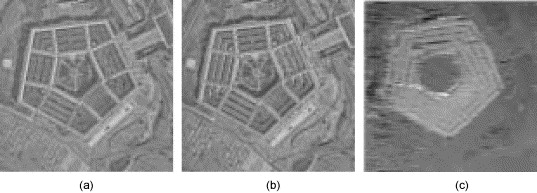
\includegraphics[scale=1.5]{4.jpg}}
\caption{Левое и среднее изображения - фотографии Пентагона. Правое - карта 
диспаратности.}
\label{pic:4}
\end{figure}

Построение карты диспаратности – сложная вычислительная задача.
Кроме того, проблема соответствия была и остается нерешенной полностью 
проблемой. Это связано со следующими причинами:
\begin{itemize}
\item \textit{Шум}. Если мы говорим о съемке в реальных, а не лабораторных условиях, 
то на получаемых фотографиях практически всегда будут присутствовать 
такие неизбежные факторы: световые блики, размытие изображения и 
просто шум, полученный из-за несовершенных сенсоров. Из этого 
следует, что алгоритмы, решающие проблему соответствия, должны быть 
устойчивыми.
\item \textit{Однотонные области}. Эта проблема также получила название проблема 
апертуры. Информация, получаемая с крайне текстурированных областей, 
должна быть распространена на однотонные области
\item \textit{Разрывность глубины}. Многие алгоритмы требуют для своей работы того, 
чтобы на некоторой области глубина была непрерывной. Это создает 
проблемы, когда в нужную область попадают границы объектов, то есть 
места, где глубина терпит разрыв.
\item \textit{Заслоненные области}. Те пиксели, которые являются заслоненными на 
одном изображении, не должны быть поставлены в соответствие пикселям
из другого изображения.
\end{itemize}

Теперь сформулируем проблему соответствия более строго. Будем считать, 
что у нас на вход дается два изображения: базовое и парное к нему. 
Определим 
$I_b = \{I(p) | p \in $ базовому изображению $\}$ 
и $I_m = \{I(p) | p \in $ парному изображению$\}$, где функция $I(p)$ – функция сопоставления пикселю изображения его интенсивности. 
Наша задача: построить карту 
диспаратности $f = \{f_p | p \in$ базовому изображению$\}$, где каждое $f_p$
представляет соответствие между пикселем $p$ базового изображения и 
пикселем $p$ - $f_p$ парного изображения. Поскольку мы полагаем, что 
изображения были предварительно ректифицированы, то $f_p$ можно 
рассматривать как скаляр, а не как двумерный вектор, и прибавление 
осуществляется к x-координате пикселя.

\section{Обзор существующих решений}
\label{other_algos}
Алгоритмы решения проблемы соответствия делятся на два класса: локальные и глобальные. Каждый из классов имеет свои плюсы и минусы, но большинство алгоритмов выполняют, частично или полностью, следующие шаги:
\begin{itemize}
\item Вычисление стоимостей соответствий. 
\item Суммирование стоимостей. 
\item Вычисление диспаратностей на основе вычисленных стоимостей. 
\item Улучшение карты диспаратности.
\end{itemize}

\subsection{Локальные алгоритмы}
\label{local}

Этот класс алгоритмов подсчитывает диспаратность каждого пикселя в отдельности, используя окна фиксированного или адаптируемого размера для корреляции. 
Алгоритмы данного класса могут быть реализованы достаточно эффективно для использования в режиме реального времени~\cite{localhirsch}. 
Однако, выбор формы окна и его размеров является непростой задачей. Это связано с тем, что, с одной стороны,
корреляция предполагает, что глубина всех пикселей внутри окна не терпит разрывов. Это
значит, что увеличение размеров окна ведет к нарушению этого условия и, как следствие, к
некорректной работе алгоритма. С другой стороны, уменьшение размеров окна ведет к
увеличению влияния шума, что приводит к уменьшению корректных совпадений. Для
локальных алгоритмов стоимость соответствия (т.е. первый шаг работы) определяется как
схожесть между двумя областями, одна из которых находится в базовом изображении, а
другая в парном. Форма этих областей зависит от конкретного алгоритма. Стандартные
подходы, появившиеся на заре исследований проблемы соответствия, используют
прямоугольное окно фиксированного размера. Размеры этого окна определяются опытным
путем. Объем вычислений, в этом случае, сильно сокращается по сравнению с современными
методами (о них позже), но существует ряд проблем, избежать которых, используя
фиксированный размер окна, практически невозможно. 

Таким образом, локальные алгоритмы обладают хорошей производительностью, но имеют низкое качество результатов.

\subsection{Глобальные алгоритмы}
\label{global}
В отличие от локальных алгоритмов, где нахождение диспаратности происходит для каждого
пикселя отдельно, целью глобального подхода является поиск наилучшей карты
диспаратности для всего изображения сразу. Глобальные методы практически всю работу
выполняют на шаге вычисления диспаратностей, часто пропуская шаг суммирования
стоимостей соответствия. Чаще всего глобальные алгоритмы решают проблему соответствия
путем минимизации функционала энергии. 

Допустим, мы хотим найти наилучшую конфигурацию $f$ . Подходящая конфигурация
будет минимизировать функционал $E$ – функционал глобальной энергии 
$$ E(f) = E_{data}(f) + \lambda  E_{smooth}(f)$$

Первое слагаемое показывает: насколько хорошо данная конфигурация согласуется с
парой входных изображений. Для того чтобы подсчитать первое слагаемое, используются
попиксельные стоимости :

$$E_{data}(f) = \sum {C(x,y, f(x,y))}$$

Второе слагаемое отвечает за штраф, налагаемый на данную конфигурацию, в случае,
когда она нарушает непрерывность диспаратностей. Чаще всего рассматриваются соседние
пиксели:

$$E_{smooth}(f)=\sum\limits_{(x,y)}  (p(f (x,y) - f(x+1,y)) + p (f(x,y) - f(x,y+1)))$$

После того, как функционал определен, существует целый ряд алгоритмов, позволяющих найти его минимум.
Классическими являются: Марковские сети, максимальный поток, graph-cuts.
 К сожалению, поиск минимума это очень сложная
вычислительная задача (поиск минимума $ E(f)$ является NP - полной задачей). Одним из
методов, призванных решить эту проблему, является динамическое программирование.
Вместо поиска минимума для всего изображения сразу, поиск ведется построчно, причем
строки обрабатываются независимо друг от друга. Такой подход применяется, например, в
\cite{maxlikelihood}. Нахождение минимума для одной строки возможно, в этом случае, за полиномиальное
время. Проблемы данного подхода очевидны, при вычислении карты диспаратностей мы
совершенно не учитываем связей между пикселями в разных строках, кроме того, этот
подход требует, чтобы относительный порядок пикселей в строке был одинаковым для левого
и правого изображения, что невозможно выполнить в том случае, когда на сцене находится
узкий объект на переднем плане.

Глобальные алгоритмы дают отличные результаты в нахождении карты
диспаратностей. Количество ошибок, допускаемых ими, относительно невелико. Тем не
менее, в настоящее время, ни один из предложенных алгоритмов, таких как $Gruph Cuts$~\cite{gruph_cuts} и $Belief Propogation$~\cite{belief_propogation}, не может быть реализован в
реальном времени на современном оборудовании, в соответствии с \cite{scharstein}. 


\section{Semi-Global Matching}
\label{sgm}
Алгоритм SGM (Semi-Global Matching) был предложен Heiko Hirschmuller 
в статье \cite{sgm}. Преимущества этого подхода, по сравнению с другими решениями, состоит в
том, что, с одной стороны, он дает очень неплохие результаты с точки зрения качества, так
как не является уже локальным алгоритмом; с другой стороны, результат достигается за
приемлиемое время.
Получение карты диспаратности алгоритмом Semi-Global Matching состоит из трех
шагов:
\begin{itemize} 
\item Вычисление попиксельной стоимости.
\item Суммирование попиксельных стоимостей.
\item Вычисление карт диспаратности.
\end{itemize}
Перед выполнением всех этих шагов необходимо вычислить интенсивности пикселей
обоих изображений. Далее все вычисления производятся с интенсивностями пикселей.
Рассмотрим каждый из шагов более подрабно:

\subsection{Вычисление попиксельной стоимости.}
Вычисление попиксильной стоимость означает присваивание некоего числа каждой паре пикселей $(p, p - d)$, где $p$ - это произвольный пиксель базового изображения, а $d$ - это число в диапозоне $[ 0, max\_disparity]$. В SGM попиксельная стоимость основана на $Census filter$ и расстоянию хэмминга, предложенние в~\cite{census}. Каждому пикселю ставится в соотвествие битовая строка на основе окна вокруг данного пикселя, где каждый бит означает больше ли интенсивность пикселя из окна, чем интенсивность самого пикселя. Затем попиксельная стоимость считается как расстояние хэмминга между соответствующими битовыми строками пикселей. 

\subsection{Суммирование попиксельных стоимостей.}
После того как вычислены попиксельные стоимости, необходимо совершить
последний шаг работы алгоритма SGM, а именно, суммирование стоимостей. Как уже
упоминалось в \ref{global} , стандартным подходом для глобальных алгоритмов является нахождение
такой конфигурации, которая минимизирует некий функционал энергии вида: 

\begin{equation}
\label{minimization}
E(f) = E_{data}(f) + \lambda  E_{smooth}(f)
\end{equation}

И как уже упоминалось, такая задача является NP-полной. Классическим
оптимизационным подходом является динамическое программирование, которое использовалось в данной задаче в статье~\cite{dp}. В этом случае
суммирование происходит вдоль одного направления, однако в этом случае связи между
пикселями в разных рядах практически, а часто и вообще, не учитываются. В \cite{sgm}  был
предложен новый подход. Суть его заключается в том, что суммирование будет происходить
одновременно по всем направлениям. Рассмотрим этот метод более подробно. 

\begin{figure}[h!]
\center{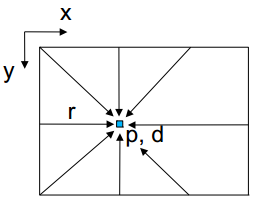
\includegraphics[scale=1.5]{5.png}}
\caption{Динамика по 8 направлениям.}
\label{pic:5}
\end{figure}

Пусть мы хотим просуммировать стоимости в направлении $r$ для данного пикселя $p$ и
диспаратности $d$. Суммирование происходит рекурсивно: 

%\begin{equation}

\begin{align}
\label{minimization2}
\begin{cases}
L_r(p, d) = C(p, d) + \min (A, B, C, D) - \min\limits_{k}  L_r(p - r, k) \\
A = L_r(p - r, d) \\
B = L_r(p - r, d + 1) + P_1 \\
C = L_r(p - r, d - 1) + P_1 \\
D = \min_{i} L_r(p - r, i) + P_2 
\end{cases}
\end{align}
%\end{equation}

Здесь первое слагаемое – это попиксельная стоимость, а второе – это минимум из
четырех чисел, которые зависят от суммированной стоимости для предыдущего пикселя в
данном направлении. $P_1$ - это константный штраф, который налагается в том случае, если
диспаратности у двух соседних пикселей отличаются на один. $P_2$ - это константный штраф,
который налагается в том случае, когда диспаратности у двух соседних пикселей отличаются
больше, чем на один. Вычитаемое слагаемое константно для всех диспаритетов пикселя p, оно необходимо для $L_r(p, d) \leq C_{max} + P_2$.

После того, как подсчитаны суммарные стоимости для каждого из направлений,
вычисляется общая сумма всех стоимостей для каждого из пикселей:
$$ S(p, d) = \sum\limits_{r} L_r(p, d)$$

Несложно заметить, что если $k$ — количество направлений, то $S \leq k (C_{max} + P_2)$.

\subsection{Вычисление карт диспаратности.}
Для каждого пикселя базового изображения p, соответствующая ему диспаратность
находится как минимум по всем диспаратностям в общем массиве стоимостей:
$$f(p) = \min\limits_{d} S(p,d)$$
В итоге получаем на выходе карту диспаратности. 

